\section{Family Ties Between 1520 and 1680}
During the timeperiod between 1520 and 1680 there were 257 men active in the Council of the Realm. As discussed earlier in subchapter \ref{councilofrealm} the council consisted mostly of men with noble background. To quantify this: according to the dataset 236 of the 257 councillors (91.8\%) were part of the ancient nobility "uradel", and only approximately 5\% were of unknown or ignoble background, most of the time bishops or other clerics.  

\begin{table}
	\caption{Absolute amount in different ranks}
	\centering
	\begin{tabular}{cccccc}
		\hline
		Commoner & Ennobled & Estate unknown & Unknown & Ancient nobility & \\
		\hline
		5 & 8 & 7 & 1 & 236 & = 257 \\
		\hline
	\end{tabular}
	\caption{Proportional amount in different ranks}
	\centering
	\begin{tabular}{cccccc}
		\hline
	    Commoner & Ennobled & Estate unknown & Unknown & Ancient nobility & \\
	    \hline
	    1.9 & 3.1 & 2.7 & 0.3 & 91.8 & $\approx$ \% \\
	\end{tabular}
\end{table}

The kingdom of Sweden was ruled by nine monarchs: Gustavus Vasa (1523-1560), Eric XIV (1560-1568), Johan III (1568-1592), Sigismund (1592-1599), Charles IX (1599-1611), Gustavus Adolphus (1611-1632), Christina (1644-1654), Carl X Gustav (1654-1660) and Carles XI (1672-1697), and two regnants from 1632 to 1654 and from 1660 to 1672 during the timeperiod. The amount of councillors appointed by each monarch\footnote{Calculated with a R script. To avoid the script dublicating the years that the monach changed, the beginning of each reign is adjusted, the actual year + 1. E. g. Eric XIV's reign is calculated 1561-1568, the actual being 1560-1668. This may cause slight inaccuracy.} or regnant varied from none to 56. Yet, 13 councillors were present before the reign of Gustavus Vasa.

The monarchs who appointed the most councillors were Gustavus Vasa (56) and queen Christina (45). The large number of councillors appointed by Gustavus Vasa may be explained by the sheer length of his reign. He ruled Sweden for 37 years, whereas all of the other monachs ruled less than 20 years. Also the religious Reformation was perfromed during his reign. The bishops and clerics that lost their position in the Council were replaced by noblement chosen by the king.\footcite[TODO]{pSuurvalta} As queen Christina ruled only for ten years, the exceptionally high number on her reign is interesting. Therefore, her reign will be discussed in greater detail in subchapter \ref{christina}. 

However, the king who appointed no new councillors was the son of Johan III: Sigismund (1566-1632). He was both the king of Poland and Sweden forming a personal union between the two countries. Why king Sigismud did not appoint any new councillors? 

\begin{figure}
	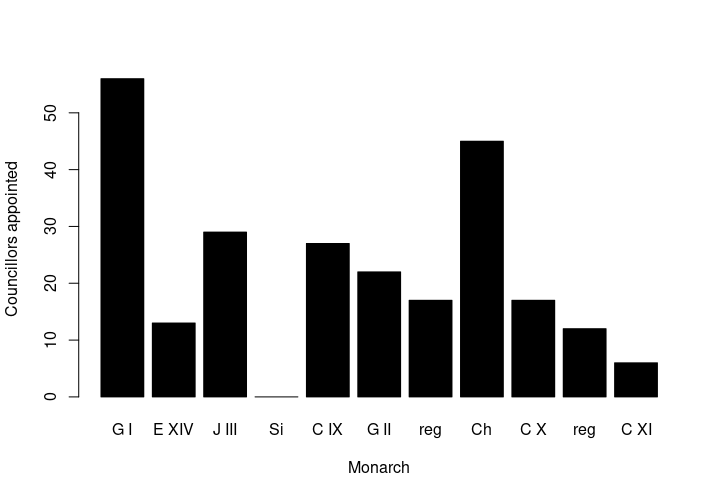
\includegraphics[scale=0.6]{councillorspermonarch.png}
	\centering
	\caption[Number of councillors appointed by each ruler between 1523-1680] {Number of councillors appointed by each monarch or regnant from 1523 to 1680. (\cite{councillorsDS}) Calculated and plotted with an R script: \url{https://github.com/Heidi-Suurkaulio/mastersthesis/blob/main/RScripts/councillors-1523-1680.R}.}
	\centering
\end{figure}

All of the councillors active between 1520 and 1680 are represented in a graph of 257 nodes and 362 edges, with self loops and parallel edges removed. The number of edges exceeds the number of nodes which means that theoretically all of the nodes could be linked to one another. Although, the edges are not distributed that way. Some of the nodes are linked to more than one other node, but some isolated nodes are indeed present. The average degree of the graph is 2.817 $\approx$ 2.8 meaning that councillors typically had 2 or 3 direct relations to another members of the Council.

The graph density is 0.011. In the mathematical definition the graph is sparse (scale from 0 to 1). However, interpretation in practical sense is not that straightforward. Having a completely dense social network, meaning that every node is directly linked to each other, is almost impossible. In this context it would mean, that each councillor is a direct relative through blood or marriage to each other, which would be weird to say at least. Further, taking the dimension of time into account, the mathematical interpretation would be even more nonsensical; how a nobleman appointed to the council in the 1670's could be directly linked to a bishop died in 1530's. 

The question wheither or not the councillors were higly linked to each other is more of a qualitative one. In the context of early modern institution, how we define a higly linked or even nepotistical institution? Probably the graph density has more explanatory value as a parameter to be compared between graphs collected from other contemporary communities.

Even so, the proportion of the nodes with at least one connection in the graph is $224/257=0.8715...$ Which means that between 1520 and 1680 the probability of a councillor being related to someone else in the Council is $\approx$ 87\%. In that sense the councillors can be considered highly networked.

Another interesting finding are the nodes with the highest and lowest degree. Maybe the most eclectic and fascinating group is the isolated nodes. There are 33 isolated nodes meaning that 33 councillors did not have any family ties within the Council. Some of them are members of the nobility with family ties to councillors active prior the beginning year of the dataset, so, the connections are excluded from this graph. These are for example: Ture Bengtsson Lilliesparre (127) or Nils Olofsson Vinge (242). Yet, some of the isolated nodes represent bishops and clerics like Magnus Sommar (186) or Ingemar Petri (162) present in the Council before the religious Reformation. 

Besides that, the isolated nodes also reveals something about the international relationships during the timeperiod. For example a teacher from France Dionysius Beurraeus (12) or a Scottish baron Robert Douglas (58) can be found. Also the famous German born chancellor Conrad von Pyhy (168) is represented as an isolated node. During his stay in Sweden von Pyhy had a significant impact on the politics of Gustavus Vasa.\footcite[p. 81-83.]{pSuurvalta} This means that as a merited foreigner one could make their way up to the Swedish Council of the Realm.

On the contrary, the nodes with the highest degree ($\geq$ 5) are of councillors who are part of the old well established aristocratic families like De la Gardie, Oxentierna, Gyllenstierna, Bielke, Stenbock, Sparre and Ribbing. Also Finnish families of Horn and Kurck can be found.\footnote{TODO} That in itself implies to the previously known fact that the aristocratic families had a remarkable stance in the negotiations and politics of the Swedish kingdom.

To focus more on the temporal dimension of the graph, I decided to divide the dataset to half. As seen in Figure \ref{fig:peryear} the most intuitive point to do the division is between years 1600 and 1601. In year 1601 duke Charles had won the civil war against king Sigismund and he practically decimated the Council of the Realm while eliminating the noblemen loyal to the former king. However, by 1602 he had to appoint 15 new councillors in order to manage the growing number of tasks in diplomacy and administration.\footcite[TODO]{pSuurvalta} By coinsidence, year 1601 also divides the timerange of the dataset in half. The firs graph depicts the network prior year 1600 and the latter one post year 1601, so, both of these represents the family ties accumulated approximately for 80 years.

\subsection{Prior 1600}
The graph depicts the family links within the Council during most of the 16th century. It consist of 111 nodes and 92 edges. In this case the number of edges subceeds the number of nodes meaning that at least some isolated nodes must be present. 

The average degree in this graph is 1.658 $\approx$ 1.7, meaning that typically councillors were directly related to one or two other members. The number is smaller than in the larger graph. However, it can be partly explained by the shorter time range, simply the family networks had not have enough time to accumulate. Thereafter, the closest comparison is the graph of councillors family ties post 1601, which will be discussed later.

The graph density is 0.015, allthough, comparing that to the bigger graph is not that straightforward. The amount of nodes having at least one connection is $85/111 = 0.765...$ meaning that the probability of councillors to be linked at least one other member is $\approx 77\%$. That is 10 percentage points smaller than in the larger graph. Even though this prior year 1600 graph is not directly comparable with the larger graph, it indicates that the family links in the 16th century were more sparse.

The amount of isolated nodes is significant: 26–as in the larger graph it was 33. The fact that, all of the bishops and clerics must be present in this graph, partly explains this. Limiting the time range also breaks some of the existing links, so for example, Pontus De la Gardie seems to be without any connections in that graph, even though his descendands were remarkably woven into the networks of Swedish aristocracy. Taking these factors into account, still the relatively high number of isolated nodes may suggest the relatively high number of incomers and larger social mobility in general.

The nodes with highest degree ($\geq$ 4) were of the remarkable noble families such as Bielke and Stenbock, however the Bååt family is more apparent in this graph than in the larger one or any of the later ones (TODO check). Did the house loose its standing somehow, or did they blend with the other noble families?

\subsubsection{the Last Man Standing: Nils Gyllenstierna}
The latter half of the 16th century and espceically the turn of the 17th century was politically turbulent time in the kingdom of Sweden. The latter half of the 16th century being affected by the rivalry between the sons of Gustavus Vasa which culminated in the civil war during the 1590's. The battle between king Sigismund and duke Charles was won by duke Charles, who later directed his spite upon the Council of the Realm. Many of the councillors were executed or fled Sweden. Despite that the Council was almost fully in devastated in 1601, one councillor was left behind: Nils Göransson Gyllenstierna (91).

Due to these circumstances, Nils Gyllenstierna had an exceptional political career. He was a nobleman born in 1526, and appointed to the Council (most likely) by Johan III in autumn 1560 at the age of 35. When he died of natural causes in 1601 at the age of 75, he had served a total of 41 years in the Council. Furthermore, he had been able to keep his position throughout all of the Gustavus Vasa's sons reigns.\footcite{councillorsDS} 

What led him to keep his position?

In fact, the last councillor to be executed in Sweden was Hogenskild Nilsson Bielke (16). He was born in 1538, and appointed to the Council by king Eric XIV in 1562 at the age of 24. He was inprisoned in Linköping in 1600 due to his incautious letters regarding duke Charles. He was executed in 1605 at the age of 67. All in all, he had served in the Council of the Realm for 36 years (being inactive for two years between 1590-1591).\footcites[p. 58.]{HakanenAKoskinen2017}{councillorsDS}

\subsection{Post Duke Charles' Revenge}
Practically, this graph begins from the year 1602 when duke Charles had to appoint 15 new councillors and the Council of the Realm was re-established. The graph consists of 146 nodes and 184 edges, now, the number of edges exceeds the number of nodes. After 1601 (or 1602) the average degree of node is 2.251 $\approx$ 2.3, larger than the 1.7 prior 1600. And, visually the graph seems more dense. 

The number of isolated nodes is significantly lower: 16, compared to the 26 prior 1600 or the 33 in the whole time period. Again it still must be remembered that limiting the time range cuts some family ties present in the dataset. Subsequently, the proportion of nodes with at least one edge is $130/146=0.890...$ ,thereby, the probability of councillor having at least one direct relation in the Council was now $\approx 89\%$. That is 12 precentage points greater than the 77\% in the 16th century, and two presentage points greater then the 87\% from the whole time period.

\begin{table}
	\caption{Number of edges needed for different densities of network}
	\label{edges}
	\begin{tabular}{cccc}
		\hline
		 & Amount of possible edges &&\\
		\hline
		density & 32 896 (all) & 6 105 (prior 1600) & 10 585 (post 1601) \\
		\hline 
		0.011 & \textbf{361.9} & 67.2 & 116.4 \\
		\hline
		0.015 & 493.5 & \textbf{91.6} & 158.8 \\
		\hline
		0.0174 & 572.4 & 106.2 & \textbf{184.2}\\
		\hline
	\end{tabular}
\end{table}

Also the density of this graph is the largest: 0.017. In prior 1600 it was 0.015 and from the whole time period 0.011. To make the denisities comparable to some degree, the amount of edges needed for different densities is counted in Table \ref{edges}. Still, the scale of the larger graph makes it hard to compare to the other graphs, so, I will focus on the two smaller ones. The graph prior 1600 would need $\approx 14$ more edges to have the density of 0.017, whereas in the graph post 1601 the difference between the density of 0.015 and 0.017 is $\approx 26$. This behaviour is explained in the subchapter \ref{network}. So, even though the time scale is similar (80 years), the density and the absolute amount of edges is different. This means that it can be argumented that the post 1601 graph is more dense than the one prior 1600. 

What the isolated nodes can tell us?

All in all, 17th century has been called in the previous literature "the century of the nobility", and the presented data seems to confirm the trend.\footnote{TODO} It seems that the family affiliations became more prominent in the Council of the Realm, and important in general, during the 17th century. Similarily, the amount of incomers decreased, which implies the slackening of social mobility.

\subsection{In the Court of Queen Christina}
\label{christina}
Queen Christina was the daughter of the king Gustavus Adolphus and queen consort Maria Eleonora of Brandenburg (1599-1655). She inherited the throne at the age of 6, after her fathers sudden death in the battlefield in November 1632. Before she was declared an adult at the age of 18 in 1644, the kingdom was ruled by a regnant.\footnote{TODO source} The reign and personal life of queen Christina are fascinating chapters in the Swedish history.\footnote{For more information see e.g. Peter Englund \textit{Silvermasken: en kort biografi över drottning Kristina} finnish version \textit{Kuningatar Kristiina}, or Marie-Louise Rodén \textit{Drottning Christina: en biografi}.}

Due that Christina's father was frequently away from Sweden and the long period of the interregnum, the authority of the Council of the Realm had grown remarkably when Christina was enthroned. Contrary to the previous monarchs, she was forced to go for the Council to get councel, yet, the situation did not stay that way for long. On the word of Hakanen and Koskinen: 

\begin{quote}
	Christina played the high nobility at their own social network game rather than enter into open warfare with them. That is, she quickly created a large group of loyal supporters around her $\dots$
\end{quote}

Furthermore, she appointed many new councillors to dilute the power of the original Council. By the year 1654 she had appointed 45 new councillors.\footcite[p. 64. ]{HakanenAKoskinen2017}

The network of councillors appointed by queen Christina is displayed in Figure \ref{queenChristinaCouncillors}. As queen Christina's reign lasted for only ten years the graph is not comparable to the other larger graphs, despite that, it is interesting in its own right. The graph consist of 45 councillors, all of them which must have been close to queen Christina in one way or another.

\begin{figure}	
	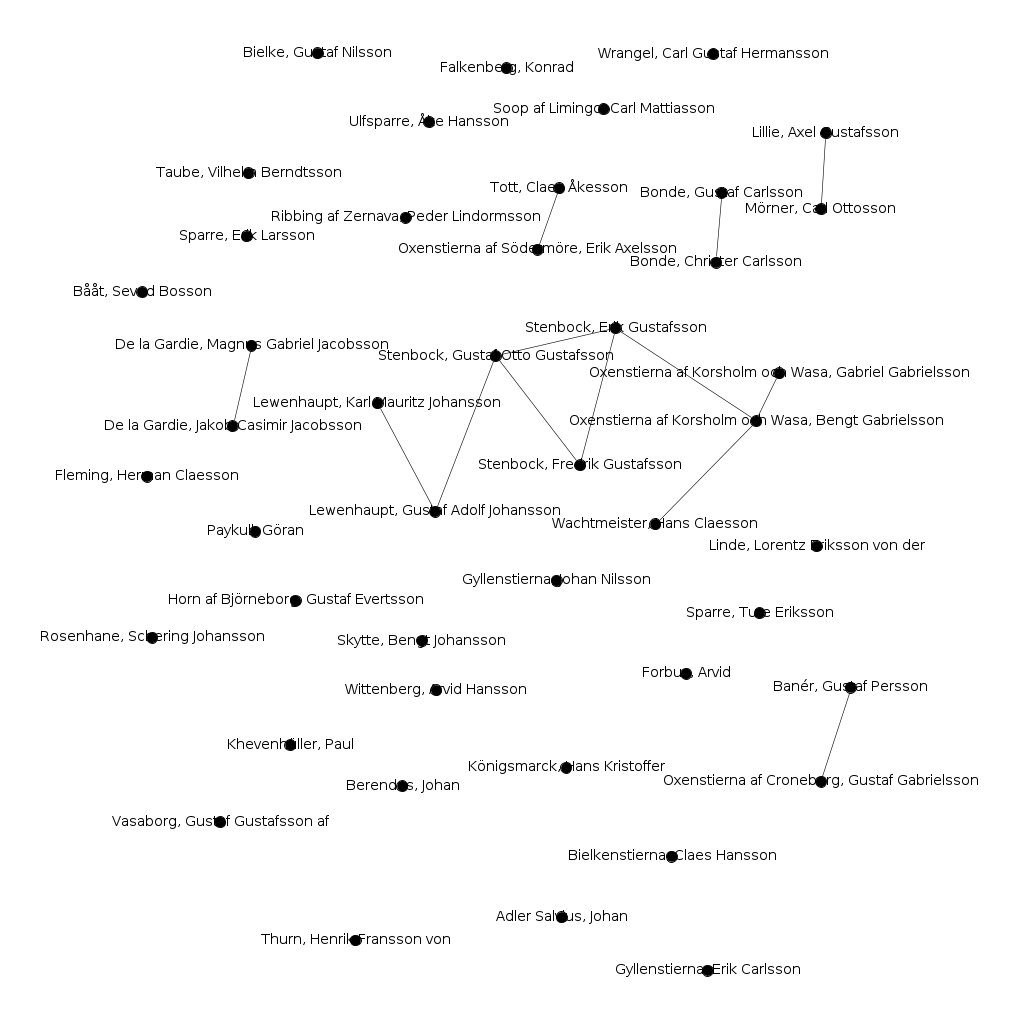
\includegraphics[width=\linewidth]{councillors_1644-1654.png}
	\caption[Councillors appointed by queen Christina]{A graph of councillors appointed by queen Christina between 1644 and 1654.(\cite{councillorsDS})}
	\label{queenChristinaCouncillors}
	\centering
\end{figure}

Overall, the network seems sparse, but, an interestingly clustered pattern can be found in the middle of the network. Eight councillors: Karl Mauritz Johansson Lewenhaupt (125), Gustaf Adolf Johansson Lewenhaupt (126), Gustaf Otto Gustafsson Stenbock (207), Fredrik Gustafssonare Stenbock (204), Erik Gustafssonall Stenbock (202), Bengt Gabrielsson Oxenstierna af Korsholm och Wasa (148), Gabriel Gabrielsson Oxenstierna af Korsholm och Wasa (154) and Hans Claesson Wachtmeister (240) are all related to each other direclty or indirectly. 

This tightly woven network seems to concentrate around the two brothers Gustaf Otto Gustafsson Stenbock and Erik Gustafssonall Stenbock. Due that they presumably had a significant position in the political life. What led them to have this position?

Some other interesting individuals can be also found on the graph. Christina appointed his paternal half brother Gustaf Gustafsson af Vasaborg (241)–Gustavus Adolphus' illegitimate son–to the Council on 5th of September 1646. Also the diplomat and nobleman Schering Johansson Rosenhane (177) who gave queen Christina the Hortus Regius -manuscript was appointed to the Council by Christina in 30th of September 1650.\footcite{councillorsDS} This may mean that family ties–even illegitimate–were of high value, but also mutual relationships had their place in the political sphere of early modern Sweden.
